\chapter{Analyse des Primitives selon le Trilemme CRO}
\epigraph{"Cryptographic primitives are the building blocks of trust in digital systems. Each must be evaluated against its resilience to emerging threats."}{- Adi Shamir}
\section{Introduction à l'Analyse CRO}
Le Trilemme CRO (Confidentialité, Fiabilité, Opposabilité) constitue un cadre d'analyse novateur pour évaluer les primitives cryptographiques dans le contexte de l'investigation numérique post-quantique. Ce chapitre applique méthodiquement ce cadre aux principales primitives cryptographiques, révélant les compromis inhérents et les optimisations possibles.

\section{Méthodologie d'Évaluation}
\subsection{Indices CRO}
Chaque primitive est évaluée selon trois indices normalisés entre 0 et 1:

\[
\text{Score CRO} = \max(C, R, O) \geq 0.4 + \text{negl}(\lambda)
\]

\begin{itemize}
\item \textbf{Confidentialité (C)}: Protection contre l'accès non autorisé
\item \textbf{Fiabilité (R)}: Intégrité, authenticité et disponibilité
\item \textbf{Opposabilité (O)}: Valeur probante en contexte juridique
\end{itemize}

\subsection{Paramètres d'Évaluation}
\begin{itemize}
\item Résistance quantique: \(\bullet\) (résistant) / \(\circ\) (vulnérable)
\item Maturité: Niveau d'adoption industrielle
\item Complexité: Coût computationnel et implémentation
\end{itemize}

\section{Analyse des Primitives Symétriques}
\subsection{AES (Advanced Encryption Standard)}
\begin{table}[H]
\centering
\begin{tabular}{lccc}
\hline
\textbf{Paramètre} & \textbf{Score} & \textbf{Justification} \\
\hline
Confidentialité (C) & 0.95 & Chiffrement robuste, résistant aux attaques classiques \\
Fiabilité (R) & 0.90 & Intégrité via modes d'opération authentifiés \\
Opposabilité (O) & 0.30 & Preuves difficilement vérifiables sans clés \\
Résistance quantique & \(\circ\) & Vulnérable à l'algorithme de Grover \\
Maturité & Élevée & Standard mondial, implémentations optimisées \\
\hline
\end{tabular}
\caption{Analyse CRO d'AES-256}
\end{table}

\subsection{ChaCha20-Poly1305}
\begin{table}[H]
\centering
\begin{tabular}{lccc}
\hline
\textbf{Paramètre} & \textbf{Score} & \textbf{Justification} \\
\hline
Confidentialité (C) & 0.93 & Performance élevée, sécurité éprouvée \\
Fiabilité (R) & 0.88 & Authentification intégrée via Poly1305 \\
Opposabilité (O) & 0.35 & Meilleure que AES mais limitations similaires \\
Résistance quantique & \(\circ\) & Vulnérable à Grover (réduction moitié) \\
Maturité & Élevée & Standardisé dans TLS 1.3, largement déployé \\
\hline
\end{tabular}
\caption{Analyse CRO de ChaCha20-Poly1305}
\end{table}

\section{Analyse des Primitives Asymétriques}
\subsection{RSA (Rivest-Shamir-Adleman)}
\begin{table}[H]
\centering
\begin{tabular}{lccc}
\hline
\textbf{Paramètre} & \textbf{Score} & \textbf{Justification} \\
\hline
Confidentialité (C) & 0.85 & Sécurité basée sur factorisation \\
Fiabilité (R) & 0.90 & Signatures robustes, standardisées \\
Opposabilité (O) & 0.95 & Excellente valeur probante, jurisprudence établie \\
Résistance quantique & \(\circ\) & Cassé par l'algorithme de Shor \\
Maturité & Très élevée & Déployé depuis 40+ ans, support universel \\
\hline
\end{tabular}
\caption{Analyse CRO de RSA-2048}
\end{table}

\subsection{ECC (Elliptic Curve Cryptography)}
\begin{table}[H]
\centering
\begin{tabular}{lccc}
\hline
\textbf{Paramètre} & \textbf{Score} & \textbf{Justification} \\
\hline
Confidentialité (C) & 0.88 & Courbes bien choisies offrent sécurité élevée \\
Fiabilité (R) & 0.92 & Signatures ECDSA largement adoptées \\
Opposabilité (O) & 0.90 & Bonne opposabilité, standards NIST \\
Résistance quantique & \(\circ\) & Vulnérable à Shor (seuil plus bas que RSA) \\
Maturité & Élevée & Adoption massive dans les systèmes modernes \\
\hline
\end{tabular}
\caption{Analyse CRO d'ECDSA avec courbe P-256}
\end{table}

\section{Analyse des Primitives Post-Quantiques}
\subsection{CRYSTALS-Kyber (KEM)}
\begin{table}[H]
\centering
\begin{tabular}{lccc}
\hline
\textbf{Paramètre} & \textbf{Score} & \textbf{Justification} \\
\hline
Confidentialité (C) & 0.92 & Sécurité basée sur LWE, résistant quantique \\
Fiabilité (R) & 0.85 & Bonnes performances, standard NIST \\
Opposabilité (O) & 0.40 & Nouvelle primitive, jurisprudence limitée \\
Résistance quantique & \(\bullet\) & Conçu spécifiquement pour résister \\
Maturité & Moyenne & Standard émergent, implémentations en cours \\
\hline
\end{tabular}
\caption{Analyse CRO de Kyber-768}
\end{table}

\subsection{CRYSTALS-Dilithium (Signatures)}
\begin{table}[H]
\centering
\begin{tabular}{lccc}
\hline
\textbf{Paramètre} & \textbf{Score} & \textbf{Justification} \\
\hline
Confidentialité (C) & 0.20 & Signatures non confidentielles par nature \\
Fiabilité (R) & 0.94 & Sécurité basée sur MLWE, robustesse élevée \\
Opposabilité (O) & 0.75 & Bon potentiel mais validation juridique nécessaire \\
Résistance quantique & \(\bullet\) & Standard NIST pour signatures PQC \\
Maturité & Moyenne & Implémentations en développement actif \\
\hline
\end{tabular}
\caption{Analyse CRO de Dilithium-3}
\end{table}

\section{Analyse des Protocoles Avancés}
\subsection{Zero-Knowledge Proofs}
\subsubsection{zk-SNARKs}
\begin{table}[H]
\centering
\begin{tabular}{lccc}
\hline
\textbf{Paramètre} & \textbf{Score} & \textbf{Justification} \\
\hline
Confidentialité (C) & 0.98 & Preuve sans révélation d'information \\
Fiabilité (R) & 0.75 & Trusted setup problématique pour l'intégrité \\
Opposabilité (O) & 0.40 & Complexité technique limite l'opposabilité \\
Résistance quantique & \(\circ\) & Vulnerable aux attaques quantiques \\
Maturité & Moyenne & Utilisation dans crypto-monnaies \\
\hline
\end{tabular}
\caption{Analyse CRO des zk-SNARKs}
\end{table}

\subsubsection{zk-STARKs}
\begin{table}[H]
\centering
\begin{tabular}{lccc}
\hline
\textbf{Paramètre} & \textbf{Score} & \textbf{Justification} \\
\hline
Confidentialité (C) & 0.85 & Transparent mais preuves volumineuses \\
Fiabilité (R) & 0.90 & Pas de trusted setup, sécurité informationnelle \\
Opposabilité (O) & 0.60 & Meilleure que SNARKs mais complexité persiste \\
Résistance quantique & \(\bullet\) & Résistance basée sur hashing \\
Maturité & Émergente & Adoption croissante, performances améliorées \\
\hline
\end{tabular}
\caption{Analyse CRO des zk-STARKs}
\end{table}

\subsection{Signatures à Seuil}
\begin{table}[H]
\centering
\begin{tabular}{lccc}
\hline
\textbf{Paramètre} & \textbf{Score} & \textbf{Justification} \\
\hline
Confidentialité (C) & 0.75 & Clés distribuées, résistance aux compromissions \\
Fiabilité (R) & 0.85 & Tolérance aux pannes, robustesse améliorée \\
Opposabilité (O) & 0.65 & Complexité administrative, processus lourd \\
Résistance quantique & Dépendante & Selon primitive sous-jacente \\
Maturité & Moyenne & Utilisation dans systèmes critiques \\
\hline
\end{tabular}
\caption{Analyse CRO des signatures à seuil (BLS)}
\end{table}

\section{Analyse Comparative}
\subsection{Tableau Synthétique des Scores CRO}
\begin{table}[H]
\centering
\resizebox{\textwidth}{!}{%
\begin{tabular}{lcccccc}
\hline
\textbf{Primitive} & \textbf{Confidentialité (C)} & \textbf{Fiabilité (R)} & \textbf{Opposabilité (O)} & \textbf{Score CRO} & \textbf{Résistance Quantique} & \textbf{Maturité} \\
\hline
AES-256 & 0.95 & 0.90 & 0.30 & 0.95 & \(\circ\) & Élevée \\
RSA-2048 & 0.85 & 0.90 & 0.95 & 0.95 & \(\circ\) & Très élevée \\
ECDSA & 0.88 & 0.92 & 0.90 & 0.92 & \(\circ\) & Élevée \\
Kyber-768 & 0.92 & 0.85 & 0.40 & 0.92 & \(\bullet\) & Moyenne \\
Dilithium-3 & 0.20 & 0.94 & 0.75 & 0.94 & \(\bullet\) & Moyenne \\
zk-SNARKs & 0.98 & 0.75 & 0.40 & 0.98 & \(\circ\) & Moyenne \\
zk-STARKs & 0.85 & 0.90 & 0.60 & 0.90 & \(\bullet\) & Émergente \\
BLS Threshold & 0.75 & 0.85 & 0.65 & 0.85 & Dépendante & Moyenne \\
\hline
\end{tabular}%
}
\caption{Comparaison des primitives cryptographiques selon le Trilemme CRO}
\end{table}

\subsection{Visualisation du Trilemme}
\begin{figure}[H]
\centering
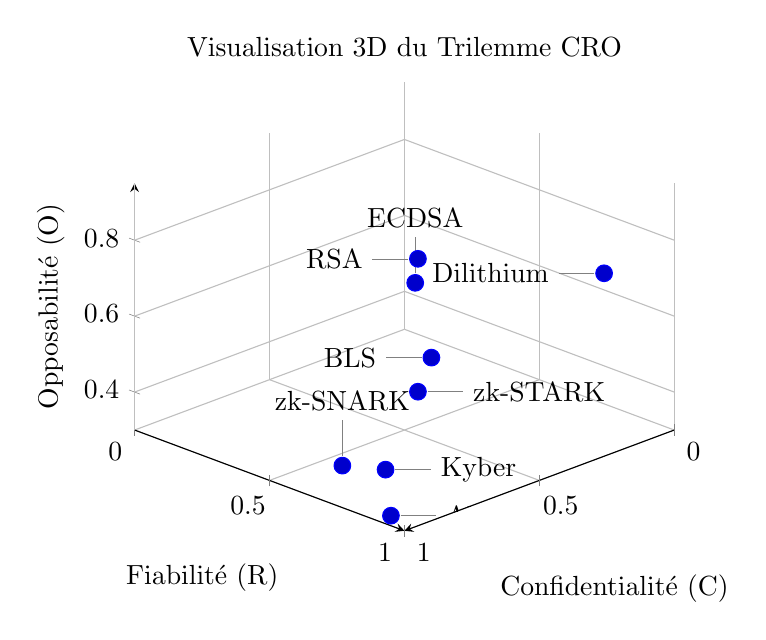
\begin{tikzpicture}
\begin{axis}[
axis lines=left,
xmin=0, xmax=1,
ymin=0, ymax=1,
xlabel=Confidentialité (C),
ylabel=Fiabilité (R),
zlabel=Opposabilité (O),
title=Visualisation 3D du Trilemme CRO,
grid=major,
view={135}{30},
]

% Points pour chaque primitive
\addplot3+[only marks,mark=*,mark size=3pt] coordinates {
(0.95,0.90,0.30) % AES
(0.85,0.90,0.95) % RSA
(0.88,0.92,0.90) % ECDSA
(0.92,0.85,0.40) % Kyber
(0.20,0.94,0.75) % Dilithium
(0.98,0.75,0.40) % zk-SNARK
(0.85,0.90,0.60) % zk-STARK
(0.75,0.85,0.65) % BLS Threshold
};

% Légende
\node at (axis cs:0.95,0.90,0.30) [pin=0:AES] {};
\node at (axis cs:0.85,0.90,0.95) [pin=180:RSA] {};
\node at (axis cs:0.88,0.92,0.90) [pin=90:ECDSA] {};
\node at (axis cs:0.92,0.85,0.40) [pin=0:Kyber] {};
\node at (axis cs:0.20,0.94,0.75) [pin=180:Dilithium] {};
\node at (axis cs:0.98,0.75,0.40) [pin=90:zk-SNARK] {};
\node at (axis cs:0.85,0.90,0.60) [pin=0:zk-STARK] {};
\node at (axis cs:0.75,0.85,0.65) [pin=180:BLS] {};

\end{axis}
\end{tikzpicture}
\caption{Représentation tridimensionnelle du Trilemme CRO pour différentes primitives}
\end{figure}

\section{Implications pour la Conception de Systèmes}
\subsection{Architectures Hybrides}
L'analyse CRO démontre la nécessité d'architectures hybrides combinant:

\begin{itemize}
\item \textbf{Primitives classiques} pour l'opposabilité juridique immédiate
\item \textbf{Primitives post-quantiques} pour la confidentialité future
\item \textbf{Protocoles avancés} pour des propriétés spécifiques
\end{itemize}

\subsection{Recommandations de Conception}
\begin{enumerate}
\item \textbf{Approche hybride}: Combiner RSA/ECC avec Kyber/Dilithium
\item \textbf{Échelonnement temporel}: 
\begin{itemize}
\item Court terme: RSA-2048 + ECDSA
\item Moyen terme: RSA-3078 + Kyber-1024
\item Long terme: Dilithium-5 + Kyber-1024
\end{itemize}
\item \textbf{Adaptation contextuelle}: Choix des primitives selon:
\begin{itemize}
\item Sensibilité des données
\item Exigences juridiques
\item Contraintes de performance
\end{itemize}
\end{enumerate}

\subsection{Implémentation du Trilemme en Pratique}
\begin{lstlisting}[language=Python, caption=Implémentation de l'analyse CRO]
class CROAnalyzer:
    """Analyseur de primitives selon le Trilemme CRO"""
    
    def __init__(self):
        self.primitive_database = self.load_primitive_data()
    
    def evaluate_primitive(self, primitive_name, context):
        """Évalue une primitive selon le contexte d'usage"""
        primitive = self.primitive_database[primitive_name]
        
        # Application des pondérations contextuelles
        weights = self.get_context_weights(context)
        
        weighted_scores = {
            'confidentiality': primitive['C'] * weights['C'],
            'reliability': primitive['R'] * weights['R'],
            'opposability': primitive['O'] * weights['O']
        }
        
        cro_index = max(weighted_scores.values())
        
        return {
            'scores': weighted_scores,
            'cro_index': cro_index,
            'quantum_safe': primitive['quantum_safe'],
            'recommendation': self.generate_recommendation(
                primitive, context, cro_index)
        }
    
    def get_context_weights(self, context):
        """Retourne les pondérations selon le contexte"""
        weights = {
            'data_protection': {'C': 0.7, 'R': 0.2, 'O': 0.1},
            'legal_evidence': {'C': 0.2, 'R': 0.3, 'O': 0.5},
            'authentication': {'C': 0.3, 'R': 0.6, 'O': 0.1},
            'long_term_archiving': {'C': 0.4, 'R': 0.4, 'O': 0.2}
        }
        return weights[context]
    
    def generate_recommendation(self, primitive, context, cro_index):
        """Génère une recommandation contextuelle"""
        if cro_index < 0.6:
            return "Primitive non recommandée pour ce contexte"
        
        recommendations = {
            'RSA-2048': "Utilisable jusqu'en 2030, migration PQC nécessaire",
            'Kyber-768': "Recommandé pour nouveaux systèmes, surveillance standardisation",
            'Dilithium-3': "Standard émergent pour signatures, évaluation juridique en cours"
        }
        
        return recommendations.get(primitive['name'], 
                                 "Évaluation spécifique requise")
\end{lstlisting}

\section{Conclusion et Perspectives}
L'analyse systématique selon le Trilemme CRO révèle plusieurs insights cruciaux:

\begin{enumerate}
\item \textbf{Aucune primitive n'optimise simultanément C, R et O}
\item \textbf{Compromis nécessaires}: Le choix doit être contextuel
\item \textbf{Urgence de la migration}: Les primitives classiques atteignent leurs limites
\item \textbf{Innovation nécessaire}: Besoin de nouvelles constructions optimisées CRO
\end{enumerate}

Les travaux futurs devront se concentrer sur:
\begin{itemize}
\item Développement de primitives optimisées CRO
Standardisation des protocoles hybrides
Cadres juridiques adaptés aux nouvelles primitives
\end{itemize}

Le Trilemme CRO offre ainsi un cadre précieux pour guider la transition vers l'investigation numérique post-quantique, en permettant des choix éclairés et contextualisés des primitives cryptographiques.